%* 
%* ------------------------------------------------------------------
%* UserManual.tex - Model Railroad System user documents
%* Created by Robert Heller on Sat Nov  9 15:33:35 2002
%* ------------------------------------------------------------------
%* Modification History: $Log$
%* Modification History: Revision 1.1  2002/11/09 21:21:07  heller
%* Modification History: Time Table User Manual
%* Modification History:
%* Modification History: Revision 1.1  2002/07/28 14:03:50  heller
%* Modification History: Add it copyright notice headers
%* Modification History:
%* ------------------------------------------------------------------
%* Contents:
%* ------------------------------------------------------------------
%*  
%*     Model RR System, Version 2
%*     Copyright (C) 1994,1995,2002  Robert Heller D/B/A Deepwoods Software
%* 			51 Locke Hill Road
%* 			Wendell, MA 01379-9728
%* 
%*     This program is free software; you can redistribute it and/or modify
%*     it under the terms of the GNU General Public License as published by
%*     the Free Software Foundation; either version 2 of the License, or
%*     (at your option) any later version.
%* 
%*     This program is distributed in the hope that it will be useful,
%*     but WITHOUT ANY WARRANTY; without even the implied warranty of
%*     MERCHANTABILITY or FITNESS FOR A PARTICULAR PURPOSE.  See the
%*     GNU General Public License for more details.
%* 
%*     You should have received a copy of the GNU General Public License
%*     along with this program; if not, write to the Free Software
%*     Foundation, Inc., 675 Mass Ave, Cambridge, MA 02139, USA.
%* 
%*  
%* 
\documentclass[12pt,notitlepage,twoside]{book}
\usepackage{epsfig}
\usepackage{mathptm}
\usepackage{times}
\usepackage{makeidx}
\usepackage{url}
\usepackage{../MyTitlepage}
\usepackage{../MyPart}
\pagestyle{headings}
\makeindex
\emergencystretch=50pt
\begin{document}
\newcommand{\MRRSubTitle}{User Manual}
%* 
%* ------------------------------------------------------------------
%* titlepage.tex - Common documentation title page
%* Created by Robert Heller on Sun Oct 13 15:59:49 2002
%* ------------------------------------------------------------------
%* Modification History: $Log$
%* Modification History: Revision 1.3  2007/10/22 17:17:27  heller
%* Modification History: 10222007
%* Modification History:
%* Modification History: Revision 1.2  2004/04/14 23:20:24  heller
%* Modification History: Updated copyright.
%* Modification History:
%* Modification History: Revision 1.1  2002/10/17 00:02:24  heller
%* Modification History: Documentation support files.
%* Modification History:
%* Modification History: Revision 1.1  2002/07/28 14:03:50  heller
%* Modification History: Add it copyright notice headers
%* Modification History:
%* ------------------------------------------------------------------
%* Contents:
%* ------------------------------------------------------------------
%*  
%*     Model RR System, Version 2
%*     Copyright (C) 1994,1995,2002  Robert Heller D/B/A Deepwoods Software
%* 			51 Locke Hill Road
%* 			Wendell, MA 01379-9728
%* 
%*     This program is free software; you can redistribute it and/or modify
%*     it under the terms of the GNU General Public License as published by
%*     the Free Software Foundation; either version 2 of the License, or
%*     (at your option) any later version.
%* 
%*     This program is distributed in the hope that it will be useful,
%*     but WITHOUT ANY WARRANTY; without even the implied warranty of
%*     MERCHANTABILITY or FITNESS FOR A PARTICULAR PURPOSE.  See the
%*     GNU General Public License for more details.
%* 
%*     You should have received a copy of the GNU General Public License
%*     along with this program; if not, write to the Free Software
%*     Foundation, Inc., 675 Mass Ave, Cambridge, MA 02139, USA.
%* 
%*  
%* 
%* 
%* $Id$  
%* 

\title{Model Railroad System \\ A collection of utilities for Model Railroaders\\ \MRRSubTitle}
\author{Robert Heller \\ Deepwoods Software \\ Wendell, MA, USA}
\date{\today}
\begin{titlepage}

\maketitle

%\begin{centering}
%\epsfig{file=../Cover1.ps} \\
%\end{centering}

\clearpage


This documentation was prepared with \LaTeX.

This document describes version 2 of the Model Railroad System package.

\vspace{.25in}



{\small Copyright \copyright 1994,1995,2002-2012 by Robert Heller D/B/A Deepwoods
Software}

\vspace{.25in}

All rights reserved.  Permission is granted to copy this document in
electronic form only, so long as it is with the software it
documents. 

The author, Robert Heller, may be contacted electronically (E-Mail) via
the following:

\begin{description}
\item[FidoNet] 1:321/153, Locks Hill BBS.
\item[InterNet] heller@deepsoft.com
\end{description}

Web site URL: {\tt http://www.deepsoft.com/}.

\thispagestyle{empty}
\setcounter{page}{0}
\clearpage

\end{titlepage}


\pagenumbering{roman}
\tableofcontents
\listoffigures
\listoftables
\cleardoublepage
%       
%%* 
%* ------------------------------------------------------------------
%* Preface.tex - Preface to the user manual
%* Created by Robert Heller on Sat Apr 21 10:32:44 2007
%* ------------------------------------------------------------------
%* Modification History: $Log$
%* Modification History: Revision 1.1  2007/05/06 12:49:40  heller
%* Modification History: Lock down  for 2.1.8 release candidate 1
%* Modification History:
%* Modification History: Revision 1.1  2002/07/28 14:03:50  heller
%* Modification History: Add it copyright notice headers
%* Modification History:
%* ------------------------------------------------------------------
%* Contents:
%* ------------------------------------------------------------------
%*  
%*     Model RR System, Version 2
%*     Copyright (C) 1994,1995,2002-2005  Robert Heller D/B/A Deepwoods Software
%* 			51 Locke Hill Road
%* 			Wendell, MA 01379-9728
%* 
%*     This program is free software; you can redistribute it and/or modify
%*     it under the terms of the GNU General Public License as published by
%*     the Free Software Foundation; either version 2 of the License, or
%*     (at your option) any later version.
%* 
%*     This program is distributed in the hope that it will be useful,
%*     but WITHOUT ANY WARRANTY; without even the implied warranty of
%*     MERCHANTABILITY or FITNESS FOR A PARTICULAR PURPOSE.  See the
%*     GNU General Public License for more details.
%* 
%*     You should have received a copy of the GNU General Public License
%*     along with this program; if not, write to the Free Software
%*     Foundation, Inc., 675 Mass Ave, Cambridge, MA 02139, USA.
%* 
%*  
%* 

\chapter*{Preface}
\markboth{PREFACE}{PREFACE}%
\addcontentsline{toc}{chapter}{Preface}
\label{chpt:Preface}
\typeout{$Id$}

This is the user manual for the Model Railroad system.  It is a ``work
in progress'' and I will be adding chapters as I write the various
self-contained ``main programs''.

%
\cleardoublepage
\pagenumbering{arabic}
%
\part{Time Table Generation Program}
%* 
%* ------------------------------------------------------------------
%* Preface.tex - Preface to the user manual
%* Created by Robert Heller on Sat Apr 21 10:32:44 2007
%* ------------------------------------------------------------------
%* Modification History: $Log$
%* Modification History: Revision 1.1  2007/05/06 12:49:40  heller
%* Modification History: Lock down  for 2.1.8 release candidate 1
%* Modification History:
%* Modification History: Revision 1.1  2002/07/28 14:03:50  heller
%* Modification History: Add it copyright notice headers
%* Modification History:
%* ------------------------------------------------------------------
%* Contents:
%* ------------------------------------------------------------------
%*  
%*     Model RR System, Version 2
%*     Copyright (C) 1994,1995,2002-2005  Robert Heller D/B/A Deepwoods Software
%* 			51 Locke Hill Road
%* 			Wendell, MA 01379-9728
%* 
%*     This program is free software; you can redistribute it and/or modify
%*     it under the terms of the GNU General Public License as published by
%*     the Free Software Foundation; either version 2 of the License, or
%*     (at your option) any later version.
%* 
%*     This program is distributed in the hope that it will be useful,
%*     but WITHOUT ANY WARRANTY; without even the implied warranty of
%*     MERCHANTABILITY or FITNESS FOR A PARTICULAR PURPOSE.  See the
%*     GNU General Public License for more details.
%* 
%*     You should have received a copy of the GNU General Public License
%*     along with this program; if not, write to the Free Software
%*     Foundation, Inc., 675 Mass Ave, Cambridge, MA 02139, USA.
%* 
%*  
%* 

\chapter*{Preface}
\markboth{PREFACE}{PREFACE}%
\addcontentsline{toc}{chapter}{Preface}
\label{chpt:Preface}
\typeout{$Id$}

This is the user manual for the Model Railroad system.  It is a ``work
in progress'' and I will be adding chapters as I write the various
self-contained ``main programs''.

%* 
%* ------------------------------------------------------------------
%* Introduction.tex - Introduction
%* Created by Robert Heller on Thu Apr 19 14:24:42 2007
%* ------------------------------------------------------------------
%* Modification History: $Log$
%* Modification History: Revision 1.1  2007/05/06 12:49:38  heller
%* Modification History: Lock down  for 2.1.8 release candidate 1
%* Modification History:
%* Modification History: Revision 1.1  2002/07/28 14:03:50  heller
%* Modification History: Add it copyright notice headers
%* Modification History:
%* ------------------------------------------------------------------
%* Contents:
%* ------------------------------------------------------------------
%*  
%*     Model RR System, Version 2
%*     Copyright (C) 1994,1995,2002-2005  Robert Heller D/B/A Deepwoods Software
%* 			51 Locke Hill Road
%* 			Wendell, MA 01379-9728
%* 
%*     This program is free software; you can redistribute it and/or modify
%*     it under the terms of the GNU General Public License as published by
%*     the Free Software Foundation; either version 2 of the License, or
%*     (at your option) any later version.
%* 
%*     This program is distributed in the hope that it will be useful,
%*     but WITHOUT ANY WARRANTY; without even the implied warranty of
%*     MERCHANTABILITY or FITNESS FOR A PARTICULAR PURPOSE.  See the
%*     GNU General Public License for more details.
%* 
%*     You should have received a copy of the GNU General Public License
%*     along with this program; if not, write to the Free Software
%*     Foundation, Inc., 675 Mass Ave, Cambridge, MA 02139, USA.
%* 
%*  
%* 

\chapter{Introduction}
\label{chapt:Introduction}
\typeout{$Id$}

This manual presents some information about how to write programs that
use various parts of Model Railroad System to control and manage various
aspects of operating your model railroad.  The Model Railroad System
includes code that interfaces with special hardware, including the PI
Engineering Raildriver Console (see
Chapter~\ref{chapt:RaildriverServer}), a Bruce Chubb network of control
nodes (see  Chapter~\ref{chapt:CMRIProgramming}), and a Lenz XPressNet
network (see Chapter~\ref{chapt:XPressNetProgramming}).  Also included
are a collection of Tcl scripts that implement a collection of widgets
that are useful for various aspects of programming utilities for a model
railroad system.

%* 
%* ------------------------------------------------------------------
%* Model Railroad System by Deepwoods Software
%* ------------------------------------------------------------------
%* Install.tex - Installing
%* Created by Robert Heller on Tue Mar  5 08:38:18 2002
%* ------------------------------------------------------------------
%* Modification History: $Log$
%* Modification History: Revision 1.1  2002/11/09 21:21:07  heller
%* Modification History: Time Table User Manual
%* Modification History:
%* ------------------------------------------------------------------
%* Contents:
%* ------------------------------------------------------------------
%*  
%*     Model RR System, Version 2
%*     Copyright (C) 1994-2002  Robert Heller D/B/A Deepwoods Software
%* 			51 Locke Hill Road
%* 			Wendell, MA 01379-9728
%* 
%*     This program is free software; you can redistribute it and/or modify
%*     it under the terms of the GNU General Public License as published by
%*     the Free Software Foundation; either version 2 of the License, or
%*     (at your option) any later version.
%* 
%*     This program is distributed in the hope that it will be useful,
%*     but WITHOUT ANY WARRANTY; without even the implied warranty of
%*     MERCHANTABILITY or FITNESS FOR A PARTICULAR PURPOSE.  See the
%*     GNU General Public License for more details.
%* 
%*     You should have received a copy of the GNU General Public License
%*     along with this program; if not, write to the Free Software
%*     Foundation, Inc., 675 Mass Ave, Cambridge, MA 02139, USA.
%* 
%*  
%* 

\chapter{Installation}
\label{chapt:Installation}

In order for this package to work you need Tcl/Tk installed on your
system.  Visit \url{http://tcl.sourceforge.net/} for information on where to
get Tcl/Tk for your system.  There are binary self-installers for
MS-Windows and MacOS, as well as source and binary distributions for
UNIX and Linux.

The code requires at least version 8.0 of Tcl/Tk.  The current stable
version of Tcl/Tk is 8.3.

Once you have downloaded and installed Tcl/Tk, you then need to put the
code files, mrrTimeTable.tcl, pkgIndex.tcl, StdMenuBar.tcl, and
MakeTimeTable.tcl along with the graphics files, DeepwoodsBanner.gif and
banner.gif, in a common directory.  Under UNIX and Linux, check the
first line mrrTimeTable.tcl and make sure you have the correct path to
your wish executable and make sure mrrTimeTable.tcl has its executable
mode bit set ({\tt chmod +x mrrTimeTable.tcl}).  Under MS-Windows, you should
already have .tcl files bound to wish, so you should already be set. 
For MacOS visit \url{http://dev.scriptics.com/software/mac/} for detailed
information.

In order to be able to create hard copy time tables, you need to
install \LaTeX.  Visit \url{http://www.tug.org/} and select the {\tt
Interesting URLs} link to find free, shareware, and commercial
distributions of \LaTeX\ for UNIX/Linux, MS-Windows, and MacOS.

If you don't have dvidvi installed on your system it is included with
this package.  You should edit the Makefile and then type {\tt make dvidvi}.
Dvidvi is useful for printing double sided documents on a single-sided
printer.  Be sure to edit MakeTimeTable.tcl to set up the paths to
various programs, if they are not on your path.  You can also set the
dvips options suitable to your preferences.






%* 
%* ------------------------------------------------------------------
%* Model Railroad System by Deepwoods Software
%* ------------------------------------------------------------------
%* SettingUp.tex - Setup
%* Created by Robert Heller on Tue Mar  5 08:39:02 2002
%* ------------------------------------------------------------------
%* Modification History: $Log$
%* Modification History: Revision 1.1  2002/11/09 21:21:07  heller
%* Modification History: Time Table User Manual
%* Modification History:
%* ------------------------------------------------------------------
%* Contents:
%* ------------------------------------------------------------------
%*  
%*     Model RR System, Version 2
%*     Copyright (C) 1994-2002  Robert Heller D/B/A Deepwoods Software
%* 			51 Locke Hill Road
%* 			Wendell, MA 01379-9728
%* 
%*     This program is free software; you can redistribute it and/or modify
%*     it under the terms of the GNU General Public License as published by
%*     the Free Software Foundation; either version 2 of the License, or
%*     (at your option) any later version.
%* 
%*     This program is distributed in the hope that it will be useful,
%*     but WITHOUT ANY WARRANTY; without even the implied warranty of
%*     MERCHANTABILITY or FITNESS FOR A PARTICULAR PURPOSE.  See the
%*     GNU General Public License for more details.
%* 
%*     You should have received a copy of the GNU General Public License
%*     along with this program; if not, write to the Free Software
%*     Foundation, Inc., 675 Mass Ave, Cambridge, MA 02139, USA.
%* 
%*  
%* 

\chapter{Setting Up}
\label{chapt:SettingUp}

When you first start up the program, it will pop up a set of dialog
boxes where it will collect some information about your layout.  This
information includes: the time frame information of your
sessions\footnote{In fast clock or ``scale'' time.}, your cab names and
color codes, your stations and the distances\footnote{In ``scale'' miles
or kilometers.}, your duplicate trackage\footnote{Typical with some
``out and back'' layouts.}, and your storage tracks.  This information
is used to create your basic train scheduling chart.  You can suppress these
pop-ups by specifying options or parameters on the command like.  See
Appendix~\ref{chapt:CLI} for more information.

\section{Saved Chart file}

The first thing you will be asked about is if you would like to load an
existing chart file.  Selecting {\tt Yes} will pop up a file selection
dialog asking for the chart file to load.  If a chart file is loaded,
the rest of the setup procedure is skipped.

\section{Session Time Frame}

If you did not load a chart file, the next thing you will be asked for
is the session time frame.  The ``Get Time Information'' dialog box
will be displayed, as shown in Figure~\ref{fig:getTimeDialog}.  The
default is 24 scale (fast clock) hours with 15 scale minute increments.
This is the horizontal dimension of the chart.  The time will be
displayed along the top in hours labeling fat vertical lines, with
thiner vertical lines at the increment value increments.

\begin{figure}
\begin{centering}
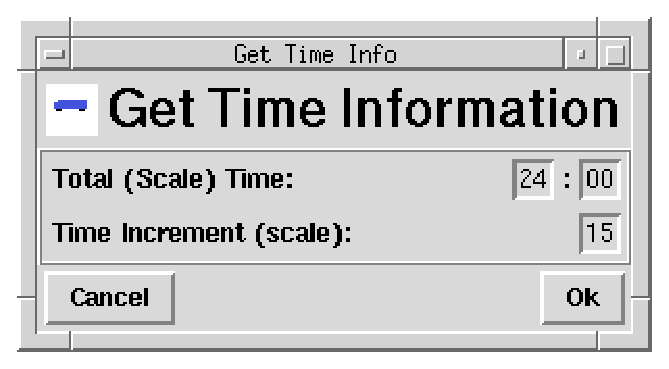
\epsfig{file=TimeTable/getTimeDialog.ps}\\
\caption{Get Time Information dialog box.}
\label{fig:getTimeDialog}
\end{centering}
\end{figure}

\section{Cab names and colors}

Next, your cab name and color information is collected by either
loading a cab file or with the ``Get Cab Info'' dialog box, as shown in
Figure~\ref{fig:getCabInfoDialog}.  The cab information is only needed
if you have an old-style switched DC cab control type of layout.  If you
are using a modern DCC type layout, you can cancel this dialog.  When
you add trains you will be asked for colors to draw the trains on the
chart, but these colors are only for ease of reference purposes.  After
loading the cabs you will have the option of saving the cab information
in a file.\footnote{See Appendix~\ref{chapt:Files} for information about
the format of this and other data files.}

\begin{figure}
\begin{centering}
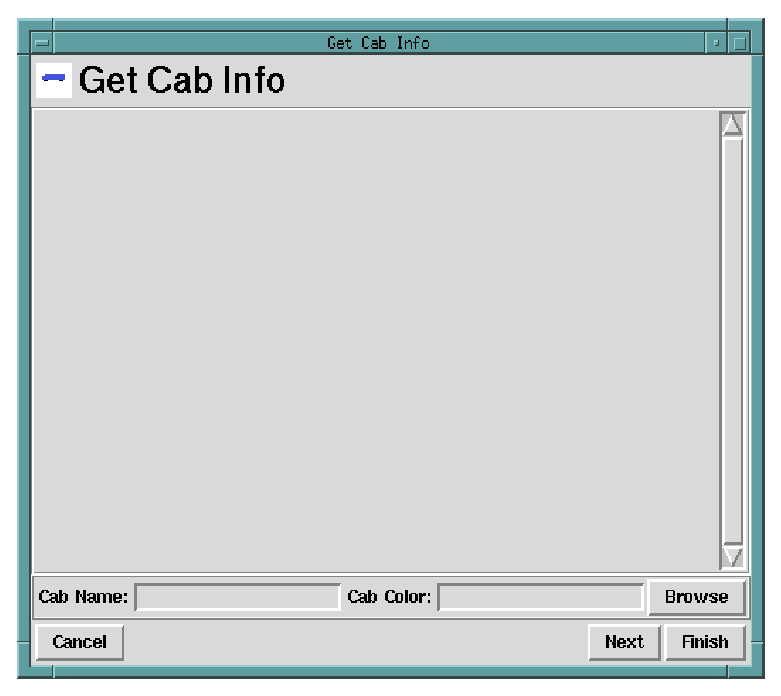
\epsfig{file=TimeTable/getCabInfoDialog.ps}\\
\caption{Get Cab Info dialog box.}
\label{fig:getCabInfoDialog}
\end{centering}
\end{figure}

\section{Getting Station List}
\label{sect:GettingStationList}

Next,  you will enter your stations and their distances down the line.
Either you can load a file with this information or you can use the
dialog box described below. 

The distances are presumed to be in $smiles$, which are scale miles
computed as shown in Equation~\ref{equ:smiles}.
\begin{equation}
Smiles = \frac{(DIS) (SF) (CR)}{5280}
\label{equ:smiles}
\end{equation}
where $(DIS)$ is the distance in real feet, $(SF)$ is your scale factor,
and $(CR)$ is your fast clock ratio.  It is possible to use
$skilometers$ instead.  These are computed as shown in
Equation~\ref{equ:skilometers}.  You will need to enter train speeds in
$skph$ instead of $smph$.
\begin{equation}
Skilometers = \frac{(DIS) (SF) (CR)}{1000}
\label{equ:skilometers}
\end{equation}
where $(DIS)$ is the distance in real meters, $(SF)$ is your scale
factor, and $(CR)$ is your fast clock ratio.

Once you have computed your station distances in $smiles$ (or
$skilometers$), you are ready to create your station list using the
``Get Station List'' dialog box, shown in
Figure~\ref{fig:getStationListDialog}.  The stations are the
vertical dimension of the chart, with the station names labeling
horizontal lines across the chart.  

\begin{figure}
\begin{centering}
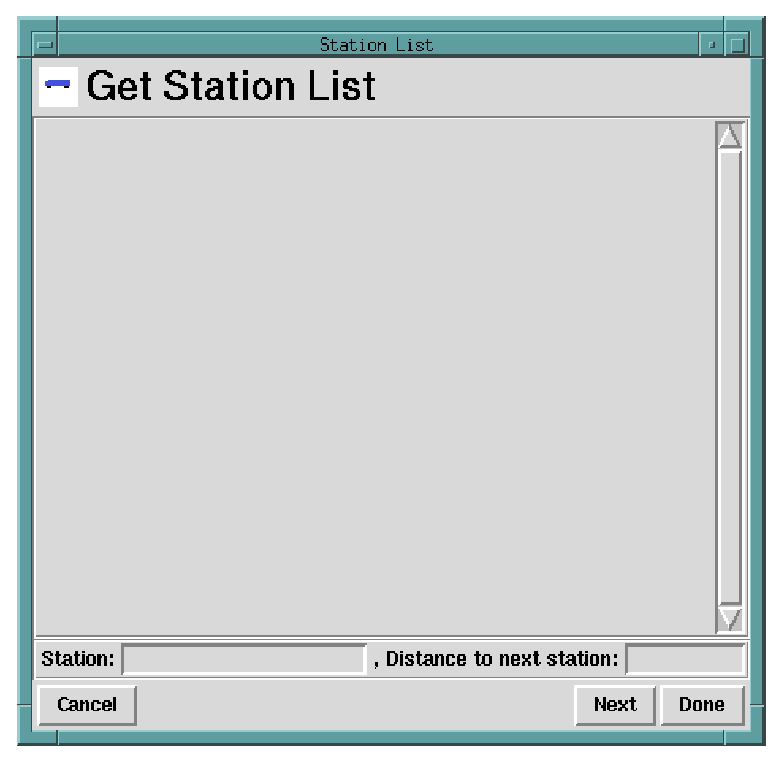
\epsfig{file=TimeTable/getStationListDialog.ps}\\
\caption{Get Station List dialog box.}
\label{fig:getStationListDialog}
\end{centering}
\end{figure}   

After getting the station list, a dialog box is presented to collect
your ``duplicate trackage''. The most common sort of duplicate trackage
occurs when you have an out and back type layout, which you are
graphing as if it is a either a continuous loop or an end-to-end
switching layout.  There is an example if Figure~8-4on page 86 of
\cite{Chubb77}. The ``Get Duplicate Trackage'' dialog box is shown in
Figure~\ref{fig:getDuplicateTrackageDialog}. Once you have entered your
stations you will have the option of saving them to a file.

\begin{figure}
\begin{centering}
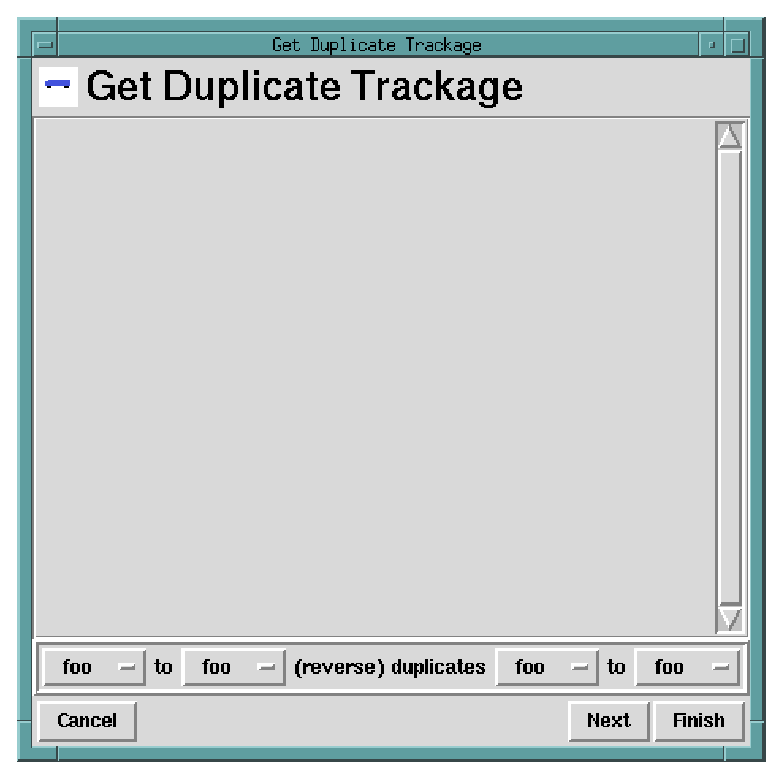
\epsfig{file=TimeTable/getDuplicateTrackageDialog.ps}\\
\caption{Get Duplicate Trackage dialog box.}
\label{fig:getDuplicateTrackageDialog}
\end{centering}
\end{figure}

Finally, you can load storage tracks from a file or use the ``Get
Storage Track'' dialog box to collect your storage tracks, as shown in
Figure~\ref{fig:getStorageTracksDialog}.  You will have the option of
saving your storage track information to a file once the information has
been entered.

\begin{figure}
\begin{centering}
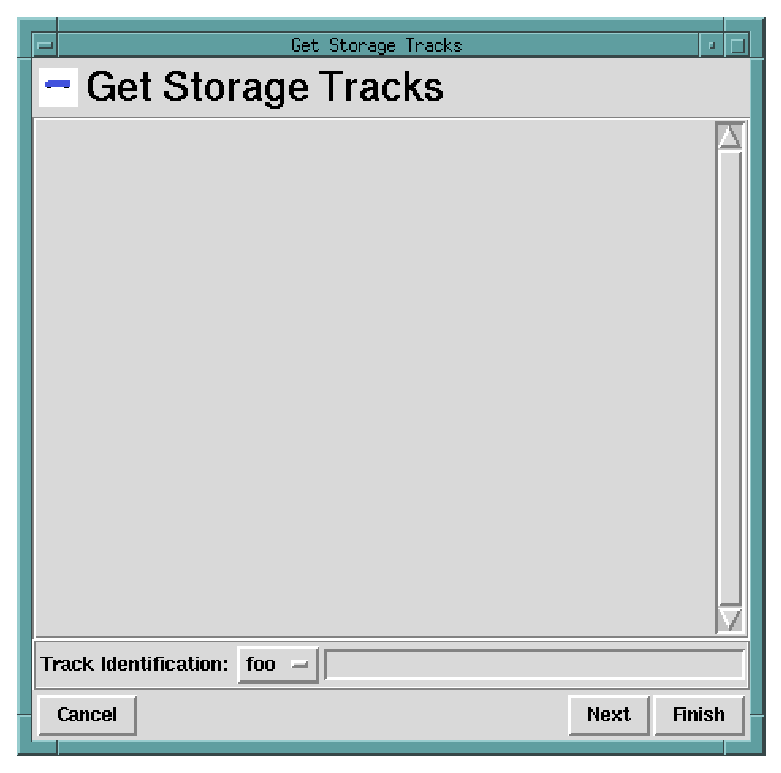
\epsfig{file=TimeTable/getStorageTracksDialog.ps}\\
\caption{Get Storage Track dialog box.}
\label{fig:getStorageTracksDialog}
\end{centering}
\end{figure}   


%* 
%* ------------------------------------------------------------------
%* Model Railroad System by Deepwoods Software
%* ------------------------------------------------------------------
%* MainGUI.tex - Main GUI
%* Created by Robert Heller on Fri Mar  8 22:43:29 2002
%* ------------------------------------------------------------------
%* Modification History: $Log$
%* Modification History: Revision 1.1  2002/11/09 21:21:07  heller
%* Modification History: Time Table User Manual
%* Modification History:
%* ------------------------------------------------------------------
%* Contents:
%* ------------------------------------------------------------------
%*  
%*     Model RR System, Version 2
%*     Copyright (C) 1994-2002  Robert Heller D/B/A Deepwoods Software
%* 			51 Locke Hill Road
%* 			Wendell, MA 01379-9728
%* 
%*     This program is free software; you can redistribute it and/or modify
%*     it under the terms of the GNU General Public License as published by
%*     the Free Software Foundation; either version 2 of the License, or
%*     (at your option) any later version.
%* 
%*     This program is distributed in the hope that it will be useful,
%*     but WITHOUT ANY WARRANTY; without even the implied warranty of
%*     MERCHANTABILITY or FITNESS FOR A PARTICULAR PURPOSE.  See the
%*     GNU General Public License for more details.
%* 
%*     You should have received a copy of the GNU General Public License
%*     along with this program; if not, write to the Free Software
%*     Foundation, Inc., 675 Mass Ave, Cambridge, MA 02139, USA.
%* 
%*  
%* 

\chapter{Main GUI}
\label{chapt:MainGUI}

Once you have loaded up your layout information, the main GUI window is
displayed, as shown in Figure~\ref{fig:mrrTTMain}.  The central portion
of the window contains your operating chart, with time along the top
from left to right and the stations along the left edge from top to
bottom.  Above the operating chart are the cabs and below the chart are
the storage tracks.  Below the chart area is a row of buttons and above
the chart is a menu bar.\footnote{Except under MacOS, where the menu bar
is wired to the top of the desktop screen.}

\begin{figure}
\begin{centering}
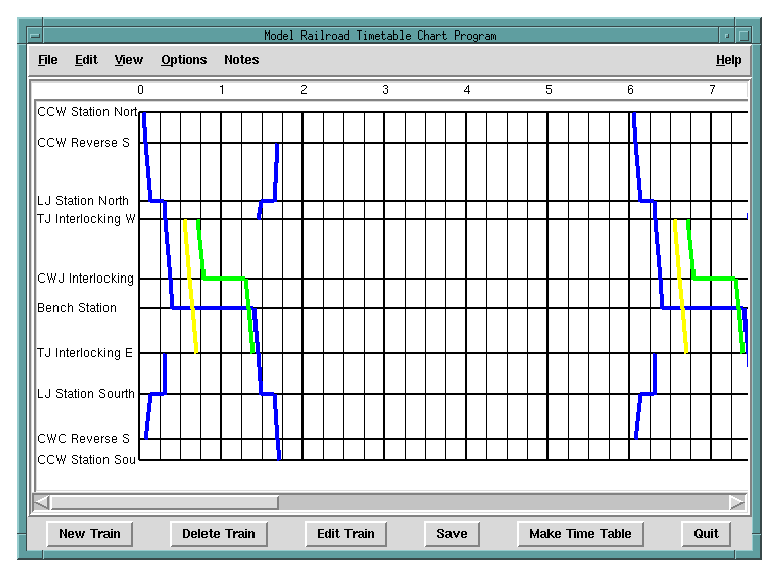
\epsfig{file=TimeTable/mrrTTMain.ps}\\
\caption{Main GUI window.}
\label{fig:mrrTTMain}
\end{centering}
\end{figure}

\section{Action Buttons}

\subsection{New Train button}

The {\tt New Train} button creates a new train.  See
Chapter~\ref{chapt:AddingTrains} for complete details on how to add a
new train.

\subsection{Delete Train Button}

The {\tt Delete Train} button is not implemented yet.

\subsection{Edit Train Button}

The {\tt Edit Train} button is not implemented yet.

\subsection{Save Button}

The {\tt Save} button saves the current file.  This is the same as the
{\tt Save} item on the {\tt File} menu.

\subsection{Make Time Table button}

The {\tt Make Time Table} button creates a hard copy time table.  See
Chapter~\ref{chapt:PrintingATimetable} for details.

\subsection{Quit button}

The {\tt Quit} button quits the application.  Same as the {\tt Close}
and {\tt Exit} items under the {\tt File} menu.


\section{Menu Bar}

\subsection{File Menu}

The {\tt File} menu follows the Motif Standard.

\subsubsection{New item}

This item clears out the current chart and creates a new one from scratch.

\subsubsection{Open\ldots\ item}

This item clears out the current chart and loads a chart saved on disk.

\subsubsection{Save item}

This item saves the current chart to the last file used to load or save
a chart.  If there is no current file, this item behaves like the {\tt
Save As\ldots} item.

\subsubsection{Save As\ldots\ item}

This item saves the current chart to a newly selected file name.

\subsubsection{Print\ldots\ item}

This item creates a hard copy time table.  See
Chapter~\ref{chapt:PrintingATimetable} for details.

\subsubsection{Close item}

This item is the same as the {\tt Exit} item and {\tt Quit} buttons.

\subsubsection{Exit item}

This item is the same as the {\tt Close} item and {\tt Quit} buttons.

\subsection{View Menu}

\subsubsection{Single Train item}

The {\tt Single Train} menu button displays the ``View Train'' pop-up
box, as shown in Figure~\ref{fig:viewSingleTrainPopup}.

\begin{figure}
\begin{centering}
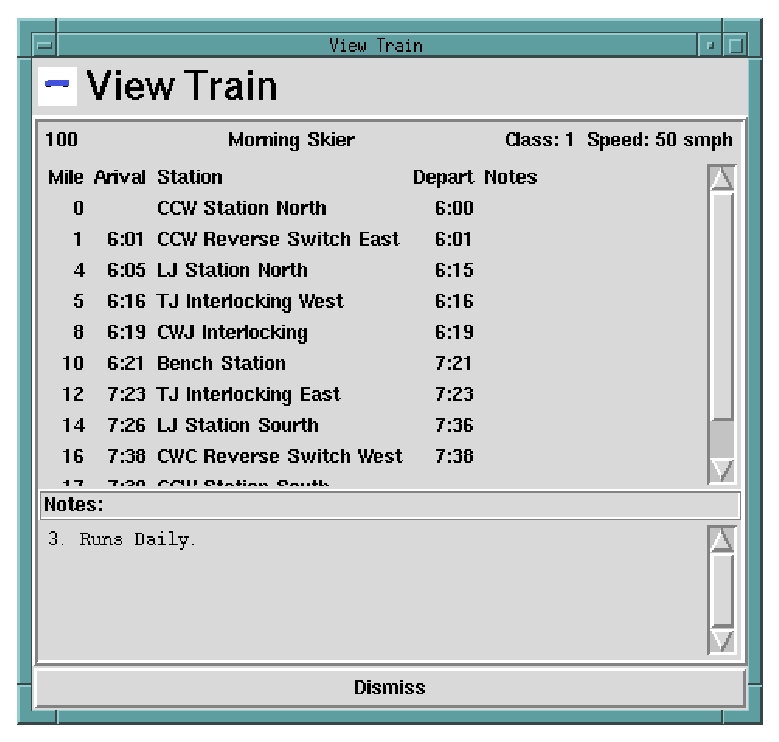
\epsfig{file=TimeTable/viewSingleTrainPopup.ps}\\
\caption{View Train Pop-up box.}
\label{fig:viewSingleTrainPopup}
\end{centering}
\end{figure}   

\subsubsection{All Trains item}

The {\tt All Trains} menu button displays the ``View All Trains'' pop-up
box, as shown in Figure~\ref{fig:viewAllTrainsPopup}. 

\begin{figure}
\begin{centering}
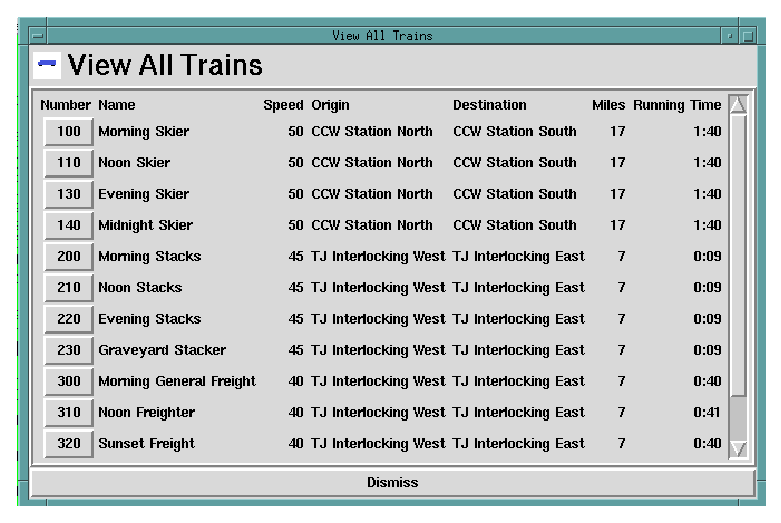
\epsfig{file=TimeTable/viewAllTrainsPopup.ps}\\
\caption{View All Trains Pop-up box.}
\label{fig:viewAllTrainsPopup}
\end{centering}
\end{figure}   

\subsubsection{Stations item}

The {\tt Stations} menu button displays the ``View Stations'' pop-up box,
as shown in Figure~\ref{fig:viewStations}.

\begin{figure}
\begin{centering}
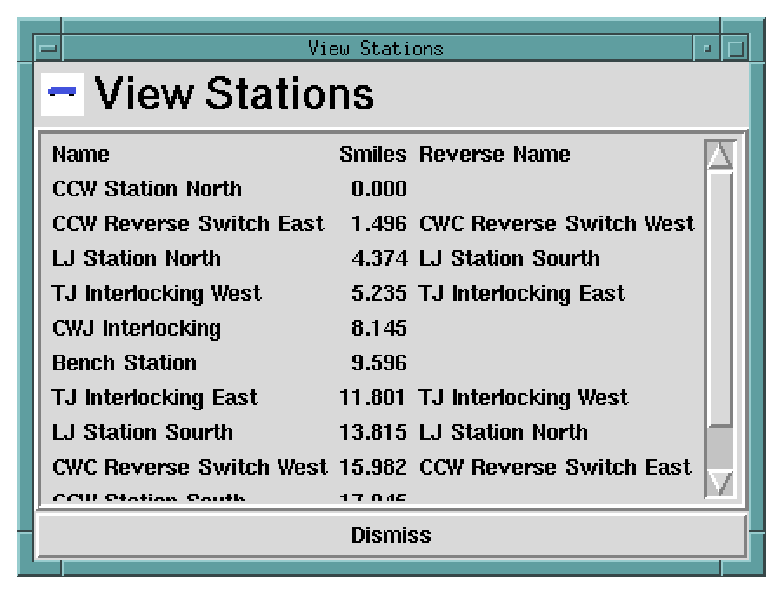
\epsfig{file=TimeTable/viewStations.ps}\\
\caption{View Stations Pop-up box.}
\label{fig:viewStations}
\end{centering}
\end{figure}   


\subsubsection{Cabs item}

The {\tt Cabs} menu button displays the ``View Cabs'' pop-up box.

\subsubsection{Storage Tracks item}

The {\tt Storage Tracks } menu button displays the ``View Storage
Tracks'' pop-up box.

\subsection{Notes Menu}

The {\tt Notes} menu is covered in Chapter~\ref{chapt:AddingNotes}.


%* 
%* ------------------------------------------------------------------
%* Model Railroad System by Deepwoods Software
%* ------------------------------------------------------------------
%* AddingTrains.tex - Adding trains
%* Created by Robert Heller on Tue Mar  5 08:39:50 2002
%* ------------------------------------------------------------------
%* Modification History: $Log$
%* Modification History: Revision 1.1  2002/11/09 21:21:07  heller
%* Modification History: Time Table User Manual
%* Modification History:
%* ------------------------------------------------------------------
%* Contents:
%* ------------------------------------------------------------------
%*  
%*     Model RR System, Version 2
%*     Copyright (C) 1994-2002  Robert Heller D/B/A Deepwoods Software
%* 			51 Locke Hill Road
%* 			Wendell, MA 01379-9728
%* 
%*     This program is free software; you can redistribute it and/or modify
%*     it under the terms of the GNU General Public License as published by
%*     the Free Software Foundation; either version 2 of the License, or
%*     (at your option) any later version.
%* 
%*     This program is distributed in the hope that it will be useful,
%*     but WITHOUT ANY WARRANTY; without even the implied warranty of
%*     MERCHANTABILITY or FITNESS FOR A PARTICULAR PURPOSE.  See the
%*     GNU General Public License for more details.
%* 
%*     You should have received a copy of the GNU General Public License
%*     along with this program; if not, write to the Free Software
%*     Foundation, Inc., 675 Mass Ave, Cambridge, MA 02139, USA.
%* 
%*  
%* 

\chapter{Adding Trains}
\label{chapt:AddingTrains}

To add a train you click on the {\tt New Train} button.  This causes the
``Create New Train'' dialog box to be displayed, as shown in
Figure~\ref{fig:createNewTrainDialog}.  This dialog box collects the
basic information about the train, such as its number, section (if any),
name (if it has one), its speed in $smph$ or $skph$, as described
in Section~\ref{sect:GettingStationList}, on
page~\pageref{sect:GettingStationList}, and the trains class, as well as
the train's originating and terminating stations.

\begin{figure}
\begin{centering}
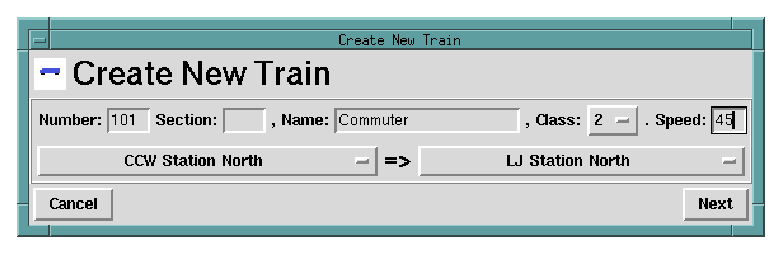
\epsfig{file=TimeTable/createNewTrainDialog.ps}\\
\caption{Create New Train Dialog box.}
\label{fig:createNewTrainDialog}
\end{centering}
\end{figure}   

Once you have entered the basic information for the train, an initial
train schedule is displayed with the ``Get Train Schedule'' dialog box,
as shown in Figure~\ref{fig:getTrainScheduleDialog}.  Initially, the
train is set to depart at midnight and make no stops and be drawn in
black (or the first cab in the (alphabetical) cab list).  The departure
times and cab/color can be changed and the {\tt Update} button clicked
on.  You can allow for layout times (for switching, etc.) by increasing
the departure time from the computed value.  Again clicking the {\tt
Update} button propagates the changes down the schedule.  Clicking {\tt
Finish} will take you to the storage track selection for departure and
arrival, if there are storage tracks at the storage tracks at the
originating or terminating stations.

\begin{figure}
\begin{centering}
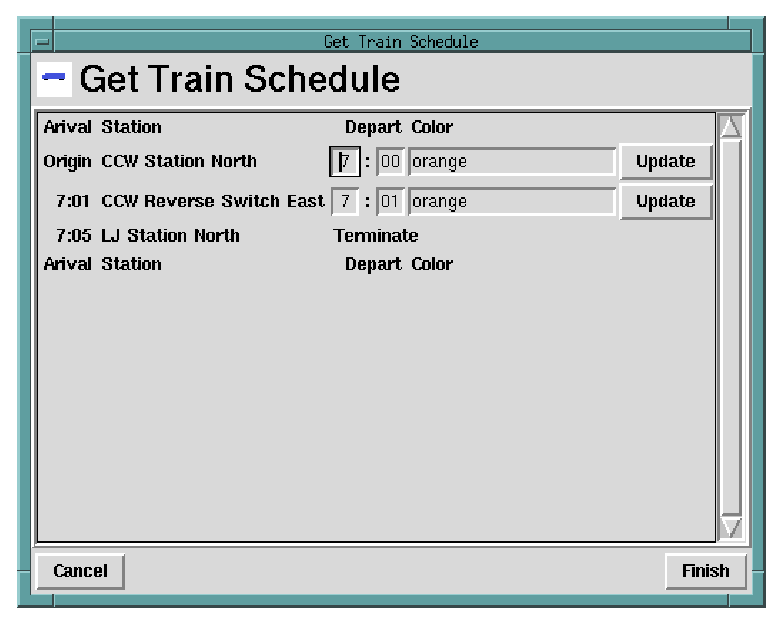
\epsfig{file=TimeTable/getTrainScheduleDialog.ps}\\
\caption{Get Train Schedule Dialog box.}
\label{fig:getTrainScheduleDialog}
\end{centering}
\end{figure}




%* 
%* ------------------------------------------------------------------
%* Model Railroad System by Deepwoods Software
%* ------------------------------------------------------------------
%* AddingNotes.tex - Adding notes
%* Created by Robert Heller on Tue Mar  5 08:40:22 2002
%* ------------------------------------------------------------------
%* Modification History: $Log$
%* Modification History: Revision 1.2  2004/04/14 23:22:17  heller
%* Modification History: Updated documentation.
%* Modification History:
%* Modification History: Revision 1.1  2002/11/09 21:21:07  heller
%* Modification History: Time Table User Manual
%* Modification History:
%* ------------------------------------------------------------------
%* Contents:
%* ------------------------------------------------------------------
%*  
%*     Model RR System, Version 2
%*     Copyright (C) 1994-2002  Robert Heller D/B/A Deepwoods Software
%* 			51 Locke Hill Road
%* 			Wendell, MA 01379-9728
%* 
%*     This program is free software; you can redistribute it and/or modify
%*     it under the terms of the GNU General Public License as published by
%*     the Free Software Foundation; either version 2 of the License, or
%*     (at your option) any later version.
%* 
%*     This program is distributed in the hope that it will be useful,
%*     but WITHOUT ANY WARRANTY; without even the implied warranty of
%*     MERCHANTABILITY or FITNESS FOR A PARTICULAR PURPOSE.  See the
%*     GNU General Public License for more details.
%* 
%*     You should have received a copy of the GNU General Public License
%*     along with this program; if not, write to the Free Software
%*     Foundation, Inc., 675 Mass Ave, Cambridge, MA 02139, USA.
%* 
%*  
%* 

\chapter{Adding, Editing, Etc. Notes}
\label{chapt:AddingNotes}

The {\tt Notes} menu manages the notes associated with a time table. 
These notes identify special conditions and situations, such as time
table variations, such as ``Sunday and Holiday'' schedules, meets, and
so on.

\section{View All Notes item}

The ``View All Notes'' menu item displays all notes currently defined. 
Each note is numbered.  A ``View All Notes'' pop-up is displayed, as
shown in Figure~\ref{fig:viewAllNotes}.

\begin{figure}
\begin{centering}
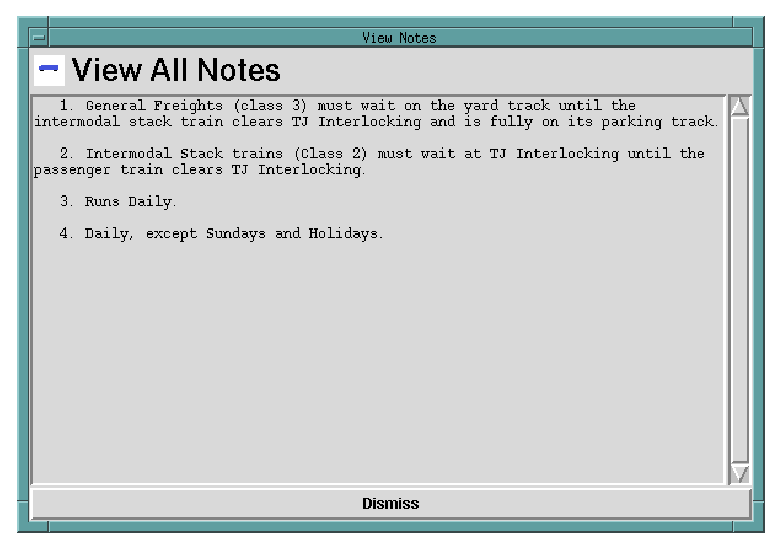
\epsfig{file=TimeTable/viewAllNotes.ps}\\
\caption{View All Notes pop-up.}
\label{fig:viewAllNotes}
\end{centering}
\end{figure}

\section{Create New Note item}
\label{sec:createNewNote}

\begin{figure}[h]
\begin{centering}
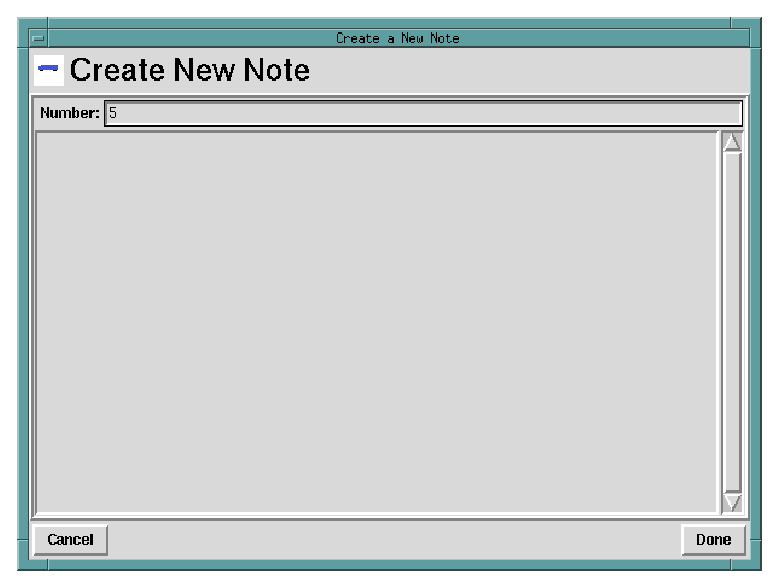
\epsfig{file=TimeTable/createNewNote.ps}\\
\caption{Create New Note dialog box.}
\label{fig:createNewNote}
\end{centering}
\end{figure} The ``Create New Note'' menu item is used to create a new
note.  The ``Create New Note'' dialog is displayed, as shown in
Figure~\ref{fig:createNewNote}.  This dialog box displays the next
available note number as a text area to enter the note in\footnote{The
note text is assumed to be \LaTeX\ code.  Normally, you can just enter
plain text, but certain characters are considered {\em spedial} to
\TeX\ and \LaTeX.  These include \%, \$, \&, \#. These characters can
be preceded with a backslash character to escape them.  On the other
hand you can include custom \LaTeX\ code to control the formatting of
your notes.}. 



\section{Delete Note item} 

The ``Delete Note'' menu item deletes a selected note.  You can only
delete notes that are not attached to a train (see
Sections~\ref{sect:addntotr} and \ref{sect:addntotrsta}).  The ``Delete
Note'' dialog box, show in Figure~\ref{fig:deleteNote}, is popped up.

\begin{figure}
\begin{centering}
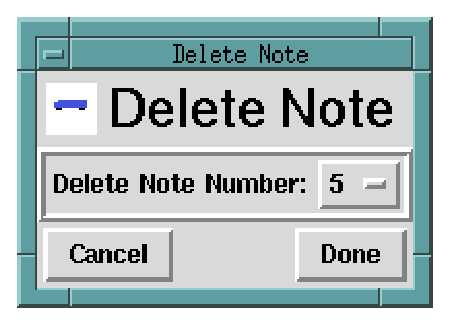
\epsfig{file=TimeTable/deleteNote.ps}\\
\caption{Delete Note dialog box.}
\label{fig:deleteNote}
\end{centering}
\end{figure}

\section{Edit Note item} 

\begin{figure}
\begin{centering}
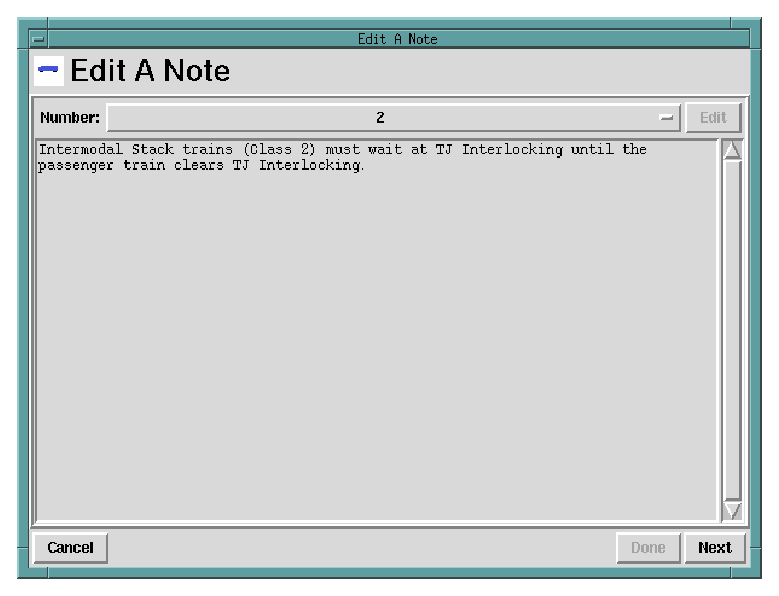
\epsfig{file=TimeTable/editNote.ps}\\
\caption{Edit Note dialog box.}
\label{fig:editNote}
\end{centering}
\end{figure} The ``Edit Note'' menu item edits a selected note. The
``Edit Note'' dialog box, show in Figure~\ref{fig:editNote}, is popped
up\footnote{See Section~\ref{sec:createNewNote}.}.



\section{Add Note To Train item} 
\label{sect:addntotr}

The ``Add Note To Train'' menu item adds a note to a train.  The note is
presumed to apply to the train as a whole, such as scheduling
restrictions, etc.  The ``Add Note To Train'' dialog box is displayed,
as shown in Figure~\ref{fig:addNoteToTrain}.

\begin{figure}
\begin{centering}
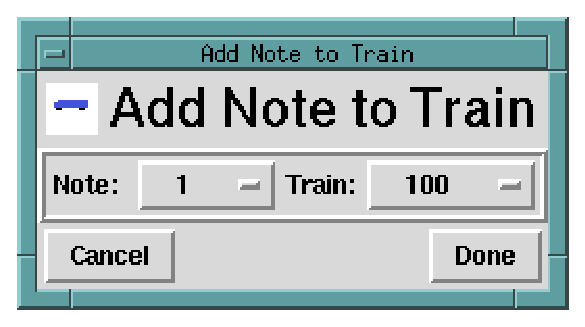
\epsfig{file=TimeTable/addNoteToTrain.ps}\\
\caption{Add Note To Train dialog box.}
\label{fig:addNoteToTrain}
\end{centering}
\end{figure}

\section{Add Note To Train at Station item}
\label{sect:addntotrsta}

The ``Add Note To Train at Station'' menu item adds a note to a train
at a specific station.  The note is presumed to apply to the train as
it is at the specified station, such as a meet or schedule switching
operations.  The ``Add Note To Train at Station'' dialog boxes are
displayed, as shown in Figures~\ref{fig:addNoteToTrainAtStation1} and
\ref{fig:addNoteToTrainAtStation2}.

\begin{figure} 
\begin{centering} 
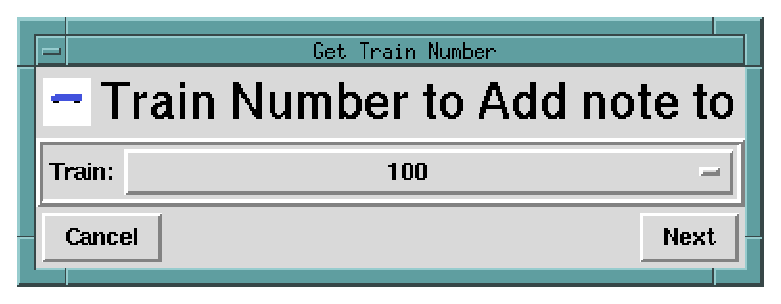
\epsfig{file=TimeTable/addNoteToTrainAtStation1.ps}\\
\caption{Add Note To Train at Station first dialog box.} 
\label{fig:addNoteToTrainAtStation1}
\end{centering} 
\end{figure}

\begin{figure} 
\begin{centering} 
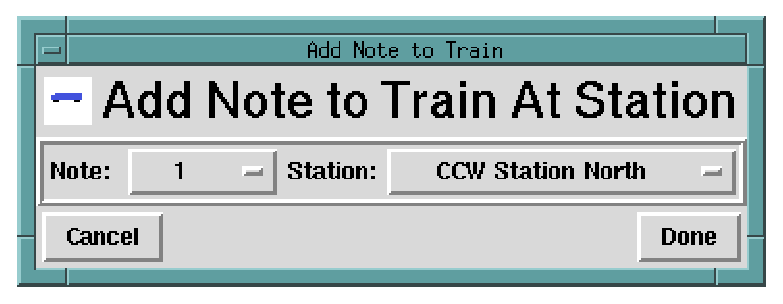
\epsfig{file=TimeTable/addNoteToTrainAtStation2.ps}\\
\caption{Add Note To Train at Station second dialog box.} 
\label{fig:addNoteToTrainAtStation2}
\end{centering} 
\end{figure}

\section{Remove Note From Train item} 

The ``Remove Note From Train'' menu item removes a note from a train.
The ``Remove Note From Train'' dialog box is displayed, as shown in
Figure~\ref{fig:removeNoteFromTrain}.

\begin{figure}
\begin{centering}
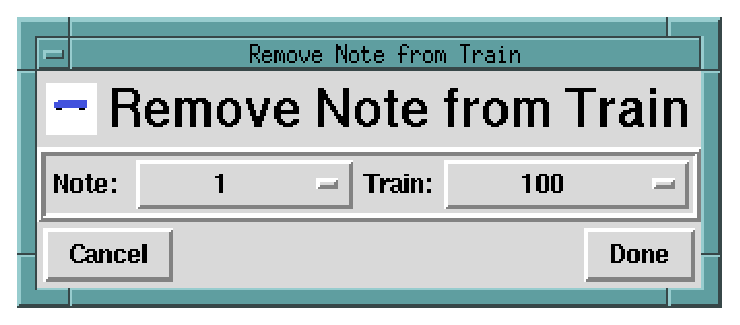
\epsfig{file=TimeTable/removeNoteFromTrain.ps}\\
\caption{Remove Note From Train dialog box.}
\label{fig:removeNoteFromTrain}
\end{centering}
\end{figure}

\section{Remove Note From Train at Station item}

The ``Remove Note From Train at Station'' menu item removes a note from
a train at a specific station. The ``Remove Note From Train at
Station'' dialog boxes are displayed, as shown in
Figures~\ref{fig:removeNoteFromTrainAtStation1} and
\ref{fig:removeNoteFromTrainAtStation2}.

\begin{figure} 
\begin{centering} 
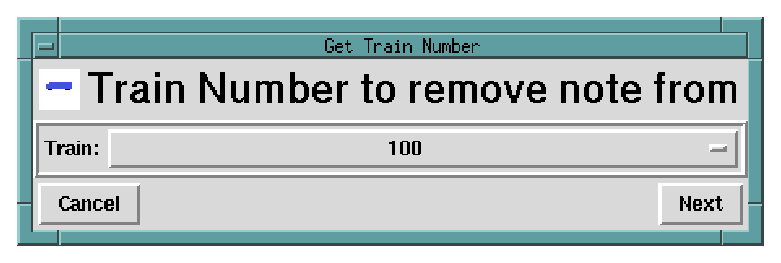
\epsfig{file=TimeTable/removeNoteFromTrainAtStation1.ps}\\
\caption{Remove Note From Train at Station first dialog box.} 
\label{fig:removeNoteFromTrainAtStation1}
\end{centering} 
\end{figure}

\begin{figure} 
\begin{centering} 
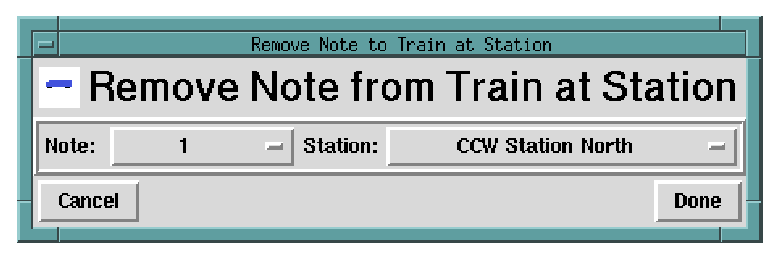
\epsfig{file=TimeTable/removeNoteFromTrainAtStation2.ps}\\
\caption{Remove Note From Train at Station second dialog box.} 
\label{fig:removeNoteFromTrainAtStation2}
\end{centering} 
\end{figure}



%* 
%* ------------------------------------------------------------------
%* Model Railroad System by Deepwoods Software
%* ------------------------------------------------------------------
%* PrintingATimetable.tex - Printing a timetable
%* Created by Robert Heller on Tue Mar  5 08:40:57 2002
%* ------------------------------------------------------------------
%* Modification History: $Log$
%* Modification History: Revision 1.2  2004/04/14 23:22:17  heller
%* Modification History: Updated documentation.
%* Modification History:
%* Modification History: Revision 1.1  2002/11/09 21:21:07  heller
%* Modification History: Time Table User Manual
%* Modification History:
%* ------------------------------------------------------------------
%* Contents:
%* ------------------------------------------------------------------
%*  
%*     Model RR System, Version 2
%*     Copyright (C) 1994-2002  Robert Heller D/B/A Deepwoods Software
%* 			51 Locke Hill Road
%* 			Wendell, MA 01379-9728
%* 
%*     This program is free software; you can redistribute it and/or modify
%*     it under the terms of the GNU General Public License as published by
%*     the Free Software Foundation; either version 2 of the License, or
%*     (at your option) any later version.
%* 
%*     This program is distributed in the hope that it will be useful,
%*     but WITHOUT ANY WARRANTY; without even the implied warranty of
%*     MERCHANTABILITY or FITNESS FOR A PARTICULAR PURPOSE.  See the
%*     GNU General Public License for more details.
%* 
%*     You should have received a copy of the GNU General Public License
%*     along with this program; if not, write to the Free Software
%*     Foundation, Inc., 675 Mass Ave, Cambridge, MA 02139, USA.
%* 
%*  
%* 

\chapter{Printing A Timetable}
\label{chapt:PrintingATimetable}

The {\tt Make Time Table} button and the {\tt Print\ldots\ } menu item
on the {\tt File} menu on the main GUI (see
Chapter~\ref{chapt:MainGUI}), creates a hard copy time table from your
chart.  This time table will list all of your trains, with arrival and
departure times at each station.

Actually, a hard copy is not directly created.  Instead, a \LaTeX\ file
is created.  Under UNIX and MS-Windows, \LaTeX\ can be run as a
subprocess, or you can manually run \LaTeX\ later.  You might even want
to edit the generated \LaTeX\ file, if you wish to add extra
information or fine tune the formatting.

\section{The first step: Time Table generation parameters}

\begin{figure}[h] 
\begin{centering} 
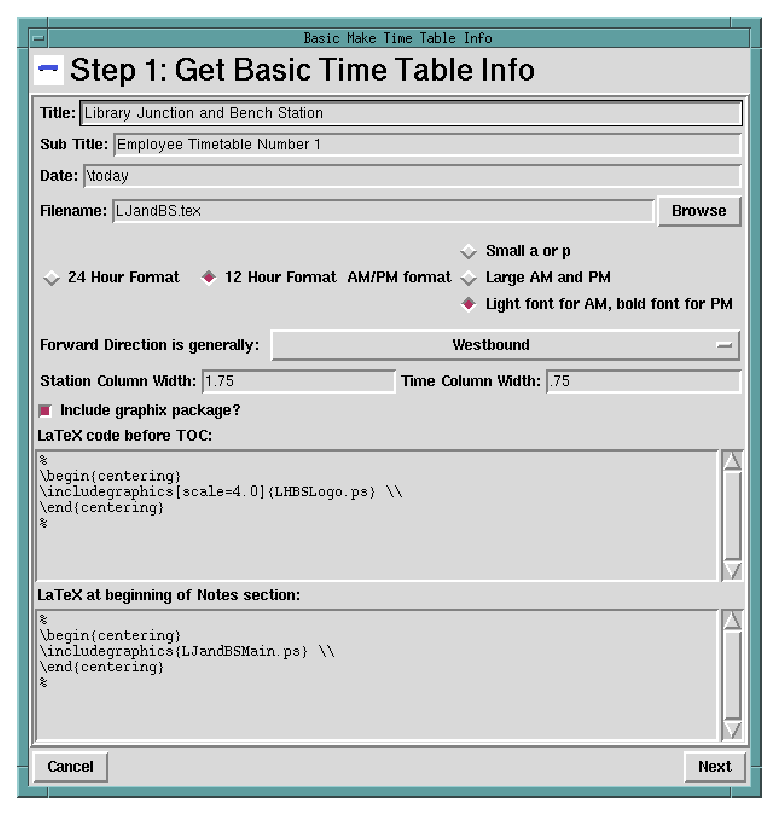
\epsfig{file=TimeTable/getBasicTimeTableInfo.ps}\\
\caption{Step 1: Get Basic Time Table Info dialog box.} 
\label{fig:getBasicTimeTableInfo}
\end{centering} 
\end{figure} When the {\tt Make Time Table} button\footnote{Or the {\tt Print\ldots\
} menu item on the {\tt File} menu.} is clicked on, you will first be
asked if you wish to load a set of previously saved Time Table
generation parameters.  After optionally loading these saved
parameters, the first (basic) set of time table generation parameters
are collected with the ``Step 1: Get Basic Time Table Info'' dialog
box, shown in Figure~\ref{fig:getBasicTimeTableInfo}.  This dialog box
collects the title, subtitle, date, filename, time format, general
layout direction and some column with information\footnote{In inches}. 
Also you can select the inclusion of the graphix \LaTeX\  package,
which allows for including graphical elements.  Also collected are
\LaTeX\ fragments to place before the Table Of Contents (such as your
railroad's logo) and to place at the beginning of the Notes section
(such as a route map).


If your time table won't fit on a single page, and unless you only run a
few trains per session, it won't, a second dialog box is pop-up after you
click {\tt Next} on the first dialog box.  The is the ``Step 2: Get
Multiple Table Time Table Info'' dialog box, shown in
Figure~\ref{fig:multipleTimeTableInfo}.  This dialog box gets
information relating to multiple pages of output, including whether to
generate single or double sided formatted output, whether to generate a
table of contents and how to group trains.

\begin{figure}
\begin{centering}
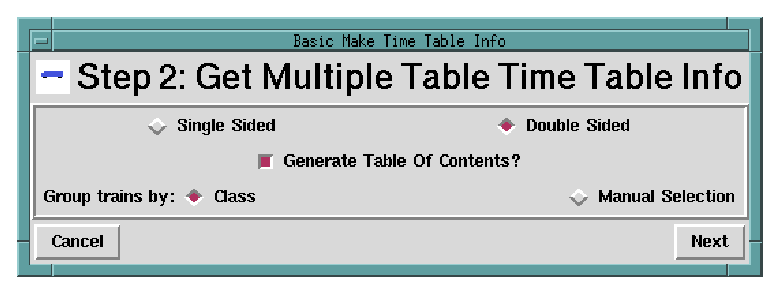
\epsfig{file=TimeTable/multipleTimeTableInfo.ps}\\
\caption{Step 2: Get Multiple Table Time Table Info dialog box.}
\label{fig:multipleTimeTableInfo}
\end{centering}
\end{figure}

\section{The second step: Grouping trains}

When printing a large set of schedules, you will be printing multiple
time tables, each for some grouping of trains.  There are two grouping
options, grouping by class and grouping manually.  Grouping by class is
easier, but only works properly if you don't have too many trains in a
given class.  Otherwise you will need to group manually.

\subsection{Grouping by class}

\begin{figure}[h]
\begin{centering}
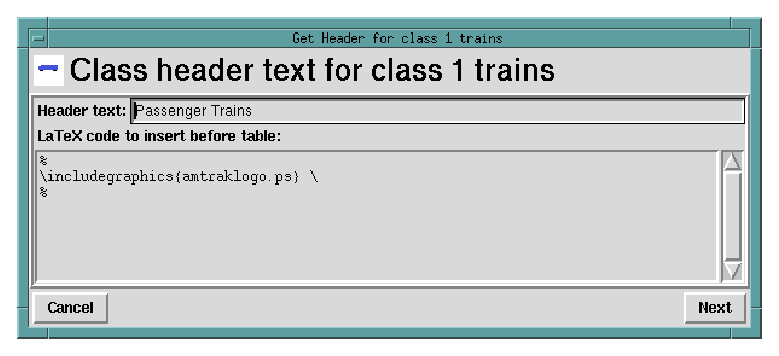
\epsfig{file=TimeTable/classGroupHeader.ps}\\
\caption{Class header text dialog box.}
\label{fig:classGroupHeader}
\end{centering}
\end{figure} When you select to group by class, a small dialog box,
like the one shown in Figure~\ref{fig:classGroupHeader}, is pop-up up
when each class is processed.  This dialog box allows you to specify a
header and some \LaTeX\ code to go at the top of the time table for the
time table for the specified class of trains.



\subsection{Grouping Manually}

When you select to group manually, the dialog box shown in
Figure~\ref{fig:manualGroup}.  This dialog box contains two lists: the
trains yet to be including in a time table and a list of trains in a
time table group.  You select one or more trains in one list and move
them to the other list using either of the \verb"<=" or \verb"=>"
buttons.  Once you have an acceptable group, you fill in the group
heading and select the {\tt Make Table} button.  Typically, a group
might be a related set of trains, such as the morning commuter trains.

\begin{figure}
\begin{centering}
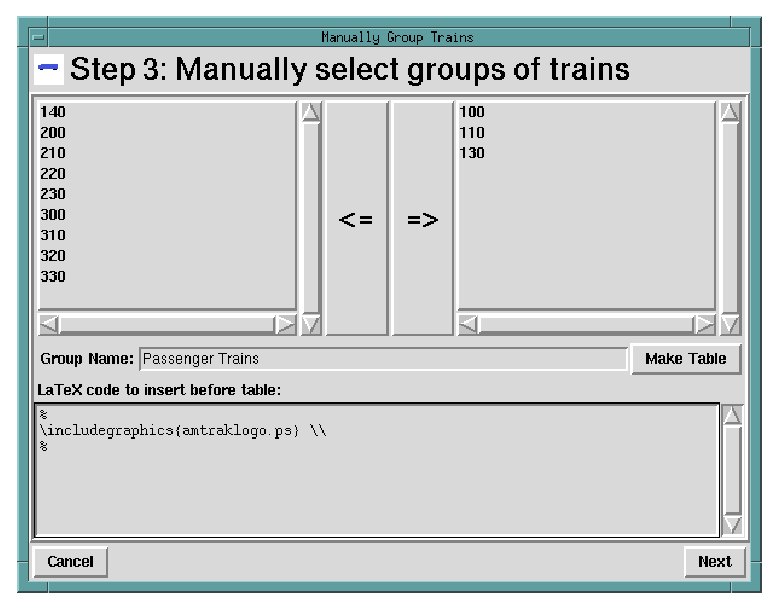
\epsfig{file=TimeTable/manualGroup.ps}\\
\caption{Manually Group Trains dialog box.}
\label{fig:manualGroup}
\end{centering}
\end{figure}   

\section{Running \LaTeX}

After the \LaTeX\ file has been generated, you will be asked if you want
to run \LaTeX.\footnote{Except under MacOS 9 or earlier.}  A series of
subprocess pop-up windows showing the progress of the subprocess runs of
\LaTeX\ and optionally dvidvi and dvips will be displayed.  You can also
skip this part and run \LaTeX\ and so on at a later time.




\appendix
%* 
%* ------------------------------------------------------------------
%* Model Railroad System by Deepwoods Software
%* ------------------------------------------------------------------
%* CommandLineArgs.tex - Command line arguments
%* Created by Robert Heller on Sat Mar  9 09:03:41 2002
%* ------------------------------------------------------------------
%* Modification History: $Log$
%* Modification History: Revision 1.1  2002/11/09 21:21:07  heller
%* Modification History: Time Table User Manual
%* Modification History:
%* ------------------------------------------------------------------
%* Contents:
%* ------------------------------------------------------------------
%*  
%*     Model RR System, Version 2
%*     Copyright (C) 1994-2002  Robert Heller D/B/A Deepwoods Software
%* 			51 Locke Hill Road
%* 			Wendell, MA 01379-9728
%* 
%*     This program is free software; you can redistribute it and/or modify
%*     it under the terms of the GNU General Public License as published by
%*     the Free Software Foundation; either version 2 of the License, or
%*     (at your option) any later version.
%* 
%*     This program is distributed in the hope that it will be useful,
%*     but WITHOUT ANY WARRANTY; without even the implied warranty of
%*     MERCHANTABILITY or FITNESS FOR A PARTICULAR PURPOSE.  See the
%*     GNU General Public License for more details.
%* 
%*     You should have received a copy of the GNU General Public License
%*     along with this program; if not, write to the Free Software
%*     Foundation, Inc., 675 Mass Ave, Cambridge, MA 02139, USA.
%* 
%*  
%* 

\chapter{Command Line Arguments}
\label{chapt:CLI}

The Time Table program command line syntax is shown in
Figure~\ref{fig:cli} and the options listed in Table~\ref{tab:cli}

\begin{figure}
\begin{centering}
\verb|./mrrTimeTable.tcl [[wish options] --] [time table options] [chartfile]|
\caption{Time Table command like syntax}
\label{fig:cli}
\end{centering}
\end{figure}

\begin{table}
\begin{centering}
\begin{tabular}{|l|p{3in}|}
\hline
Option &Description \\
\hline
\hline
-totaltime time & Specifies the total fast clock time for an operating session.\\
-timeincrement time & Specifies the fast clock time increment for the chart.\\
-cabfile file & Specifies the name of a file containing cab names and colors.\\
-nocabfile & Specifies that there are no cabs.\\
-stationfile file & Specifies the name of a file containing station
names and distances.\\
-trackfile file & Specifies the name of a file containing storage tracks.\\
-notrackfile & Specifies that there are no storage tracks.\\
\hline
\end{tabular}
\caption{Time Table Options}
\label{tab:cli}
\end{centering}
\end{table}


%* 
%* ------------------------------------------------------------------
%* Model Railroad System by Deepwoods Software
%* ------------------------------------------------------------------
%* Files.tex - Data file formats
%* Created by Robert Heller on Sat Mar  9 09:34:43 2002
%* ------------------------------------------------------------------
%* Modification History: $Log$
%* Modification History: Revision 1.1  2002/11/09 21:21:07  heller
%* Modification History: Time Table User Manual
%* Modification History:
%* ------------------------------------------------------------------
%* Contents:
%* ------------------------------------------------------------------
%*  
%*     Model RR System, Version 2
%*     Copyright (C) 1994-2002  Robert Heller D/B/A Deepwoods Software
%* 			51 Locke Hill Road
%* 			Wendell, MA 01379-9728
%* 
%*     This program is free software; you can redistribute it and/or modify
%*     it under the terms of the GNU General Public License as published by
%*     the Free Software Foundation; either version 2 of the License, or
%*     (at your option) any later version.
%* 
%*     This program is distributed in the hope that it will be useful,
%*     but WITHOUT ANY WARRANTY; without even the implied warranty of
%*     MERCHANTABILITY or FITNESS FOR A PARTICULAR PURPOSE.  See the
%*     GNU General Public License for more details.
%* 
%*     You should have received a copy of the GNU General Public License
%*     along with this program; if not, write to the Free Software
%*     Foundation, Inc., 675 Mass Ave, Cambridge, MA 02139, USA.
%* 
%*  
%* 

\chapter{Data File Formats}
\label{chapt:Files}

All data files used by this program are plain text files.  The can be
edited with a plain text editor, although this is not recommended in
general.

\section{Cabs File}

Cab files have an extension of \verb=.cabs=, and are formatted one cab
per line as shown in Figure~\ref{fig:cabfile}.

\begin{figure}
\begin{centering}
\verb=cab name|cab color=\\
\caption{Cab File line syntax}
\label{fig:cabfile}
\end{centering}
\end{figure}

\section{Stations File}

Station files an extension of \verb=.stations=, and are formatted with
the first line containing the total end-to-end run length in $smiles$
(or $skilometers$), followed by each station as shown in
Figure~\ref{fig:stationFileStations}, then comes the duplicate trackage
map as shown in Figure~\ref{fig:stationFileDupTracks}, which is flagged
by a line consisting of \verb=%%% Duplicate Trackage Map=.

\begin{figure}   
\begin{centering}
\verb=station|distance=
\caption{Station line in the Stations file}
\label{fig:stationFileStations}
\end{centering}
\end{figure}

\begin{figure}   
\begin{centering}
\verb"station=station|station=station"
\caption{Duplicate Trackage line in the Stations file}
\label{fig:stationFileDupTracks}
\end{centering}
\end{figure}


\section{Storage Track List File}

Storage Track files have an extension of \verb=.tracks=, and are
formatted one station per line as shown in Figure~\ref{fig:trackfile}.

\begin{figure}
\begin{centering}
\verb=station|track list=\\
\caption{Storage Track File  line syntax}
\label{fig:trackfile}
\end{centering}
\end{figure}


\section{Chart File}

Chart files have an extension of \verb=.chart=, and are formatted as a
series of sections, set off by lines beginning with three percent signs
(\verb=%%%=).  The first section is the time scale section, formatted
as shown in Figure~\ref{fig:chtimescale}.  Then the cab color section,
headed with the line, \verb=%%%CABCOLORS:= and then formatted as shown
in Figure~\ref{fig:cabfile}, then the station list, headed with a line
containing the total length, formatted as
\verb=%%%STATIONTOTALLENGTH:length=, followed by lines formatted as in
Figure~\ref{fig:stationFileStations}.  This is followed by the
duplicate track map, set off by the line \verb=%%%DUPLICATETRACKMAP:=
with lines formatted as in Figure~\ref{fig:stationFileDupTracks}.  Then
comes the storage tracks, headed by the line \verb=%%%STORAGETRACKS:=
with lines formatted as in Figure~\ref{fig:trackfile}.  After this
comes the trains, which are set off with the line \verb=%%%TRAINS:= and
formatted as in Figure~\ref{fig:chfileTrains}.  Then comes the storage
track usage map, headed by the line \verb=%%%STORAGETRACKMAP:= with
lines formatted as shown in Figure~\ref{fig:chfileStorUseMap}. See the
Internals Manual for details on the format of the train array and the
storage track usage map array.  Finally the notes are stored after a
heading line of \verb=%%%NOTES:= as lines formatted as in
Figure~\ref{fig:chfileNotes}. The note entries have had their internal
new line characters replaced by the two character sequence \verb=\n=.

\begin{figure}
\begin{centering}
\verb=%%%TIMESCALE: TotalTime TimeIncrement=\\
\caption{Time scale line in Chart file}
\label{fig:chtimescale}
\end{centering}
\end{figure}

\begin{figure}
\begin{centering}
\verb=train|train structure=\\
\caption{Train line in chart file}
\label{fig:chfileTrains}
\end{centering}
\end{figure}

\begin{figure}
\begin{centering}
\verb=storage key|storage usage=\\
\caption{Storage Track Usage line in chart file}
\label{fig:chfileStorUseMap}
\end{centering}
\end{figure}

\begin{figure}
\begin{centering}
\verb=note number|note text=\\
\caption{Note line in chart file}
\label{fig:chfileNotes}
\end{centering}
\end{figure}




\cleardoublepage
\addcontentsline{toc}{chapter}{Bibliography}
\bibliography{../MRR}
\bibliographystyle{plain}
\cleardoublepage
\addcontentsline{toc}{chapter}{Index}
\printindex
\end{document}

